\begin{frame}{(3) Runtime Adaptation}
  \only<1>{
    \begin{figure}
      \centering
      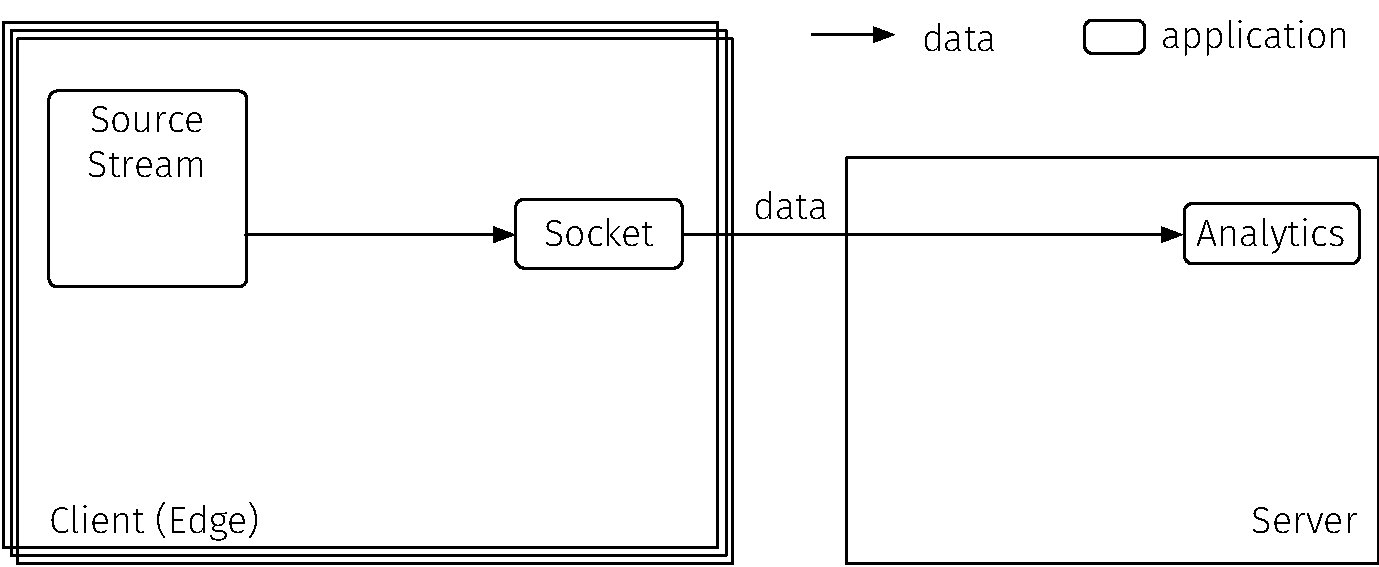
\includegraphics[width=\linewidth]{figures/runtime-arch-original.pdf}
    \end{figure}
  }
  \only<2->{
    \begin{figure}
      \centering
      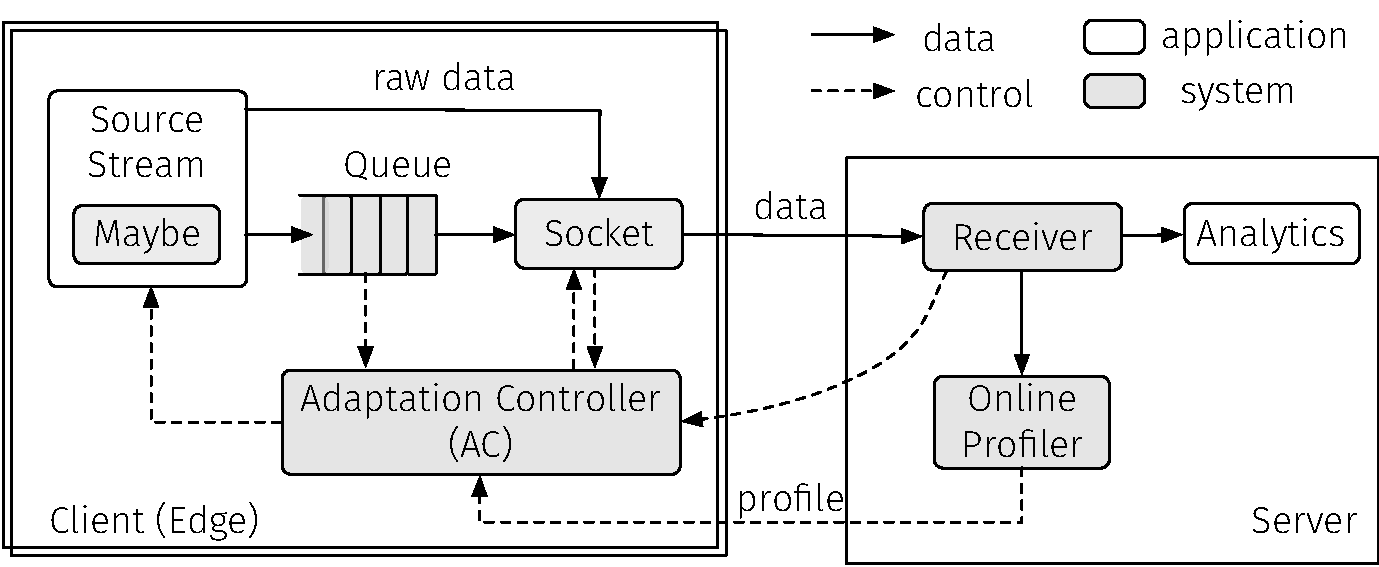
\includegraphics[width=\linewidth]{figures/runtime-arch-after.pdf}
    \end{figure}
  }

  \visible<3->{
    \begin{figure}
      \centering
      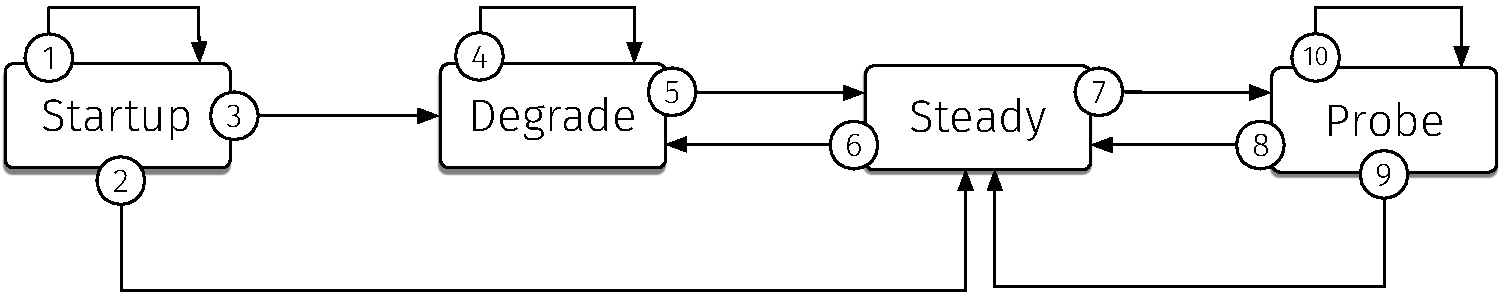
\includegraphics[width=0.8\linewidth]{figures/runtime-arch-statemachine.pdf}
      \caption{Adaptation Controller State Machine. We introduce \texttt{Probe}
        phase to conservatively change adaptation level. For details, please see
        the paper/thesis.}
    \end{figure}
  }
\end{frame}

%%% Local Variables:
%%% mode: latex
%%% TeX-master: "../talk"
%%% TeX-engine: xetex
%%% End:
